\documentclass[a4paper,11pt,french]{article}

%\usepackage[utf8]{inputenc}
%\usepackage[latin1]{inputenc}
%\usepackage[french]{babel}
\usepackage[table]{xcolor}
\usepackage{fancyhdr}
\usepackage{tabularx}
\usepackage{longtable}
\usepackage[pdftex]{graphicx}  


\usepackage[utf8x]{inputenc}
\usepackage[francais]{babel}
\usepackage[T1]{fontenc}

\begin{document}

\title{Le manuel de GuiPG}
\author{Pierre \bsc{Balmelle}, Lucas \bsc{Barbay}, Mathieu \bsc{Fin}, \\ Ibrahima \bsc{Sory Barry}, Olivier \bsc{Thibault}}
\maketitle

\normalsize
\clearpage
\tableofcontents
\clearpage

\section{Introduction}

GuiPG est une interface graphique pour utiliser le format PGP, un outil de chiffrement. GnuPG (aussi connu sous le nom de gpg) est inclus dans la plupart des distributions et est probablement installé sur votre système. Avec GuiPG, vous pourrez éditer vos clefs, mais aussi chiffrer et déchiffrer vos fichiers. L'édition de clefs vous permettra
de créer votre réseau de confiance avec la possibilité de changer la confiance d'une clef ou encore de la signer.
GuiPG vous permettra donc d'utiliser les principales commandes de GnuPG si vous n'êtes pas familiers avec le terminal.

\section{Présentation de l'interface}

Voici l'interface de GuiPG : \bigbreak

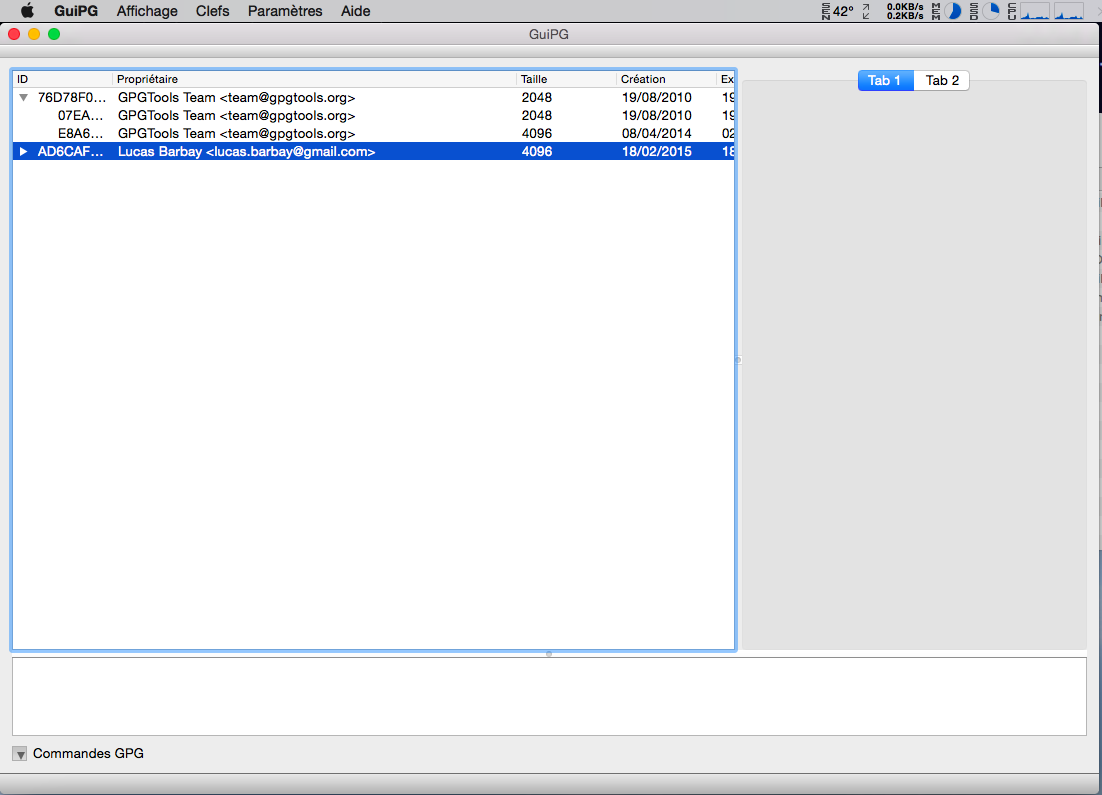
\includegraphics[scale=0.3]{interface.png} \bigbreak

Vous pouvez voir sur ce trousseau les liens de confiance que l'on peut avoir avec les clefs.

\smallbreak

L'interface est divisée en deux parties :
\begin{itemize}
\item Une partie centrale qui nous permettra de lister les clefs de notre trousseau ainsi que ses sous-clefs et les signatures. Cette liste est représentée sous forme d'arbre pour mieux visualiser les sous-clefs.
\item Une partie console en bas qui listera les commandes à chaque fois qu'une action GnuPG sera lancée par le biais de l'interface.
\end{itemize}

\section{Utilisation de GuiPG}

\subsection{Gestion des profils}

Vous pouvez utiliser plusieurs profils dans GuiPG. Chaque profil est constitué d'un nom, d'un chemin vers GPG ainsi que de la version utilisée. Cela permet d'utiliser différentes versions de GPG (1.4 ou 2) compatibles avec GuiPG et d'avoir plusieurs trousseaux de clefs. La fenêtre de gestion de profil est la suivante et permet la création, suppression ou le chargement d'un profil. \bigbreak

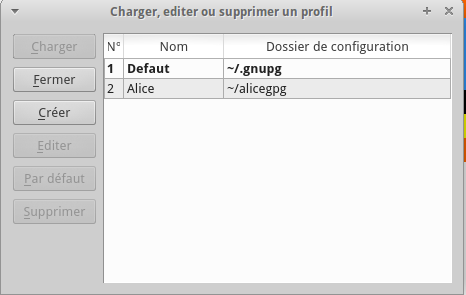
\includegraphics[scale=0.5]{profil.png}


\subsection{Création d'une clef GPG}


La fenêtre permettant de générer une clef est accessible depuis l'onglet Clefs puis Générer une paire de clefs ou depuis l'icône de création de clefs.
\bigbreak

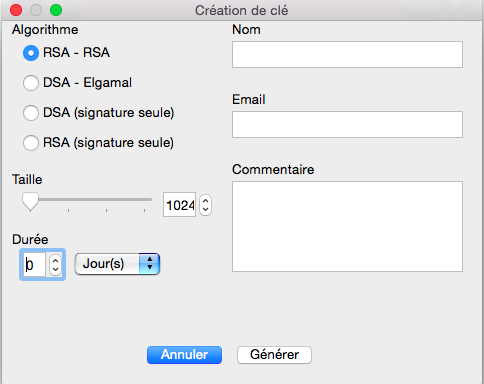
\includegraphics[scale=0.5]{creation.png} \bigbreak


Dans cette fenêtre, il faut remplir les différents champs qui constitueront la clef (le nom, l'adresse mail et optionnellement un commentaire). 
Vous avez le choix de garder les paramètres de génération par défaut ou bien de choisir l'algorithme de chiffrement, la taille de la clef ou encore
la durée de validité de celle-ci. Si vous avez peur de perdre votre mot de passe, il est conseillé de ne pas mettre une durée illimitée pour votre clef
ou de créer un certificat de révocation.


\subsection{Édition de clefs}

La vue des clefs se fait à travers un arbre permettant une meilleure visibilité des sous-clefs et signature liée aux clefs de votre trousseau. Un clic droit sur ces items permet de voir les actions possibles à travers un menu. Les actions ne sont pas les mêmes en fonction de l'item sélectionné, par exemple pour une clef, les actions possibles sont :

\begin{itemize}
\item Ajouter un identifiant utilisateur
\item Exporter la clef publique ou la clef secrète
\item Ajouter une sous-clef
\item Signer
\item Supprimer la clef
\item Modifier la confiance (Sans avis, aucune, légère, complète, ultime)
\end{itemize}

\subsection{Importation/Exportation de clefs}
L'exportation se fait à travers le menu de sélection de clefs. Vous pouvez exporter la clef publique ou la clef privée de la clef que vous venez de sélectionner.
L'importation se fait soit par le biais du menu Clefs, soit par l'icône de la toolbar. L'importation doit être utilisée sur un fichier contenant une clef.

\subsection{Cryptographie sur un fichier}

GuiPG vous permet de chiffrer un fichier à l'aide d'une clef. Il suffit de passer par le menu cryptographie et d'aller dans "Chiffrer un fichier".
L'interface permettant de chiffrer un fichier est la suivante :

\bigbreak
\bigbreak

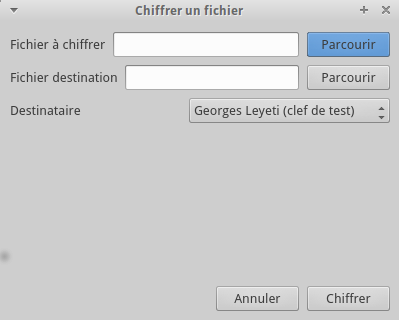
\includegraphics[scale=0.5]{chiffrer.png} \bigbreak

Pour chiffrer un fichier, vous devez donc choisir le fichier à chiffrer, choisir le répertoire de destination et choisir le destinataire du fichier chiffré.

Pour déchiffrer ou vérifier un fichier que l'on vous a envoyé, il faut également indiquer le fichier source et de destination : 

\bigbreak
\bigbreak

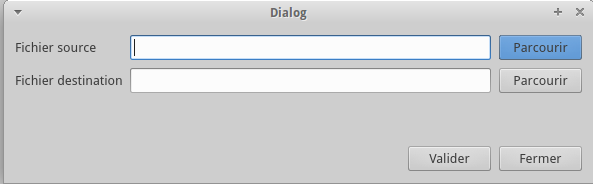
\includegraphics[scale=0.5]{dechiffrer.png} \bigbreak


\end{document}